\noindent

\includegraphics[height=1.25cm]{images/pictograms/replication}

\includegraphics[height=1.25cm]{images/pictograms/benchmark}

\includegraphics[height=1.25cm]{images/pictograms/under_construction}

\includegraphics[height=1.25cm]{images/pictograms/FDM}
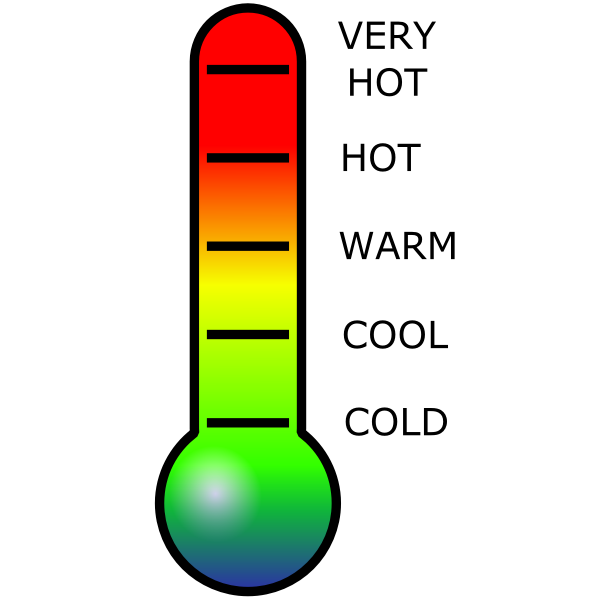
\includegraphics[height=1.25cm]{images/pictograms/temperature}

\includegraphics[height=1.25cm]{images/pictograms/paraview}
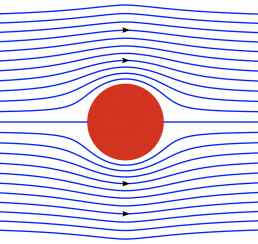
\includegraphics[height=1.25cm]{images/pictograms/streamfunction}


%%%%%%%%%%%%%%%%%%%%%%%%%%%%%%%%%%%%%%%%%%%%%%%%%%%%%%%%%%%%%%%%%%%%%%%%%%%%%%%%%%%%%%%%%%%%%%%%%%%

\begin{flushright} {\tiny {\color{gray} python\_codes/fieldstone\_155/text.tex}} \end{flushright}

%\lstinputlisting[language=bash,basicstyle=\small]{python_codes/template_keywords.key}

\par\noindent\rule{\textwidth}{0.4pt}

\begin{center}
\inpython
{\small Code: \url{https://github.com/cedrict/fieldstone/tree/master/python_codes/fieldstone_155}}
\end{center}

\par\noindent\rule{\textwidth}{0.4pt}

{\bf \color{teal} Purpose}: implement and document bla bla 

\par\noindent\rule{\textwidth}{0.4pt}

%%%%%%%%%%%%%%%%%%%%%%%%%%%%%%%%%%%%%%%%%%%%%%%%%%%%%%%%%%%%%%%%%%%%%%%%%%%%%%%%%%%%%%%%%%%%%%%%%%%


This benchmark deals with the 2-D thermal convection of a fluid 
of infinite Prandtl number in a rectangular closed cell.
In what follows, I carry out the case 1a, 1b, and 1c experiments as shown in 
Blankenbach \etal (1989) \cite{blbc89}:
steady convection with constant viscosity in a square box.

The temperature is fixed to zero on top and to $\Delta T$ at the bottom, 
with reflecting symmetry at the sidewalls (i.e. $\partial_x T=0$) 
and there are no internal heat sources. 
Free-slip conditions are implemented on all boundaries. 


$L_x=L_y=1$,
and I run the model with $Ra=10^4,10^{5}$ and $10^6$.

The initial temperature field is given by 
\begin{equation}
T(x,y)=(1-y) - 0.01\cos(\pi x) \sin(\pi y)
\end{equation}
The perturbation in the initial temperature fields leads to 
a perturbation of the density field and sets the fluid in motion. 
Depending on the initial Rayleigh number, the system ultimately reaches a 
steady state after some time. 
Note that at t=0, we have
\[
\frac{\partial T}{\partial x} = 0.01 \pi \sin(\pi x)
\]

The Nusselt number (i.e. the mean surface temperature gradient over 
mean bottom temperature)
is computed as follows \cite{blbc89}:
\begin{equation}
\Nunb = L_y \frac{\int_0^{L_x} \frac{\partial T}{\partial y}(y=L_y) \; dx  }{\int_0^{L_x} T(y=0) \; dx}
\label{eqNu}
\end{equation}
Note that in our case the denominator is equal to 1 since $L_x=1$ 
and the temperature at the bottom is prescribed to be 1.

If no convection is taking place (i.e. $\Ranb$ is too low) then 
only diffusion is taking place 
and the steady state temperature field is then $T(y)=1-y$, 
so that $\partial_y T=-1$ and we find that the Nusselt number is simply 1.

In the end, the system of coupled steady-state equations to solve is:

\begin{eqnarray}
\vec\nabla^2 \omega &=& \Ranb \frac{\partial T}{\partial x} \\
\vec\nabla^2 \Psi   &=&  -\omega \\
\vec\nabla^2 T      &=&  \vec\upnu \cdot \vec\nabla T
\end{eqnarray}

Since we are looking for the steady state 
solution and this will involve iterations, 
I have decided (for now\footnote{as an experiment}) 
to keep the advection term of the 
energy equation in the rhs, so I then must solve: 

\begin{eqnarray}
\vec\nabla^2 \omega^{k} &=& \Ranb \frac{\partial T^{k-1}}{\partial x} \\
\vec\nabla^2 \Psi^{k}   &=&  -\omega^{k} \\
\vec\nabla^2 T^k        &=& \vec\upnu^k \cdot \vec\nabla T^{k-1}
\qquad \text{with} \qquad 
\vec\upnu^k=(\partial \Psi^k/\partial y,-\partial \Psi^k / \partial x)
\end{eqnarray}
where the upperscript $k$ denotes the iteration counter.

%%%%%%%%%%%%%%%%%%%%%%%%%%%%%%%%%%%%%%%%%%
\section*{Boundary conditions}

We have three PDEs to solve. All three showcase the 
Laplace operator. We wish to prescribe free slip 
boundary conditions on all four sides of the domain. 
As documented in \stone~\ref{f153}, 
We then impose $\omega=0$ on all sides (first PDE), 
and $\Psi=0$ on all sides (second PDE). 

Concerning the temperature equation, 
we prescribe $T=1$ at the bottom and $T=0$ at the top. 
We also prescribe $\partial T/\partia x=0$ on the sides.


%%%%%%%%%%%%%%%%%%%%%%%%%%%%%%%%%%%%%%%%%%
\section*{Code structure}


Inside the time stepping loop the following five steps are necessary
\begin{enumerate}
\item solve vorticity equation
\item solve stream function equation
\item compute velocity field
\item solve temperature equation
\item compute temperature gradient
\end{enumerate}


\newpage
\begin{center}
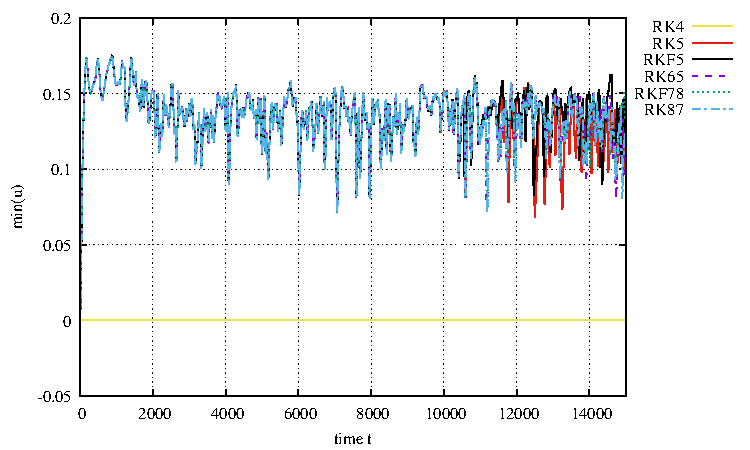
\includegraphics[width=5.7cm]{python_codes/fieldstone_155/stats_u}
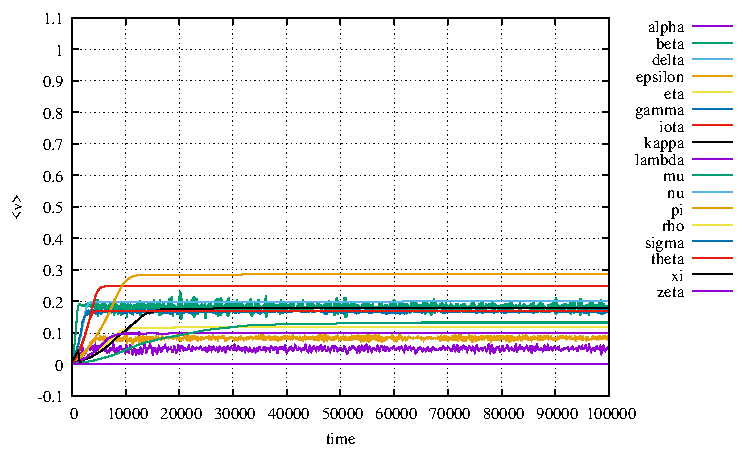
\includegraphics[width=5.7cm]{python_codes/fieldstone_155/stats_v}
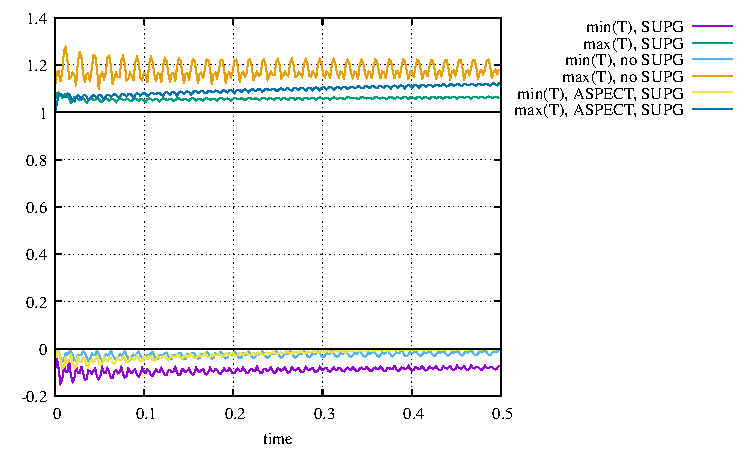
\includegraphics[width=5.7cm]{python_codes/fieldstone_155/stats_T}\\
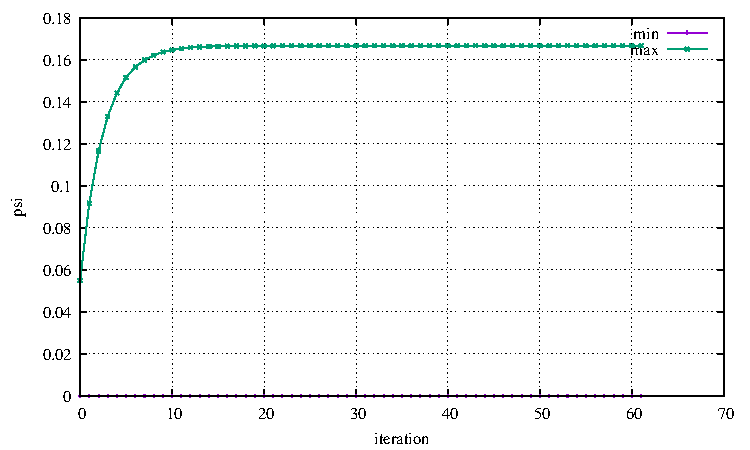
\includegraphics[width=5.7cm]{python_codes/fieldstone_155/stats_psi}
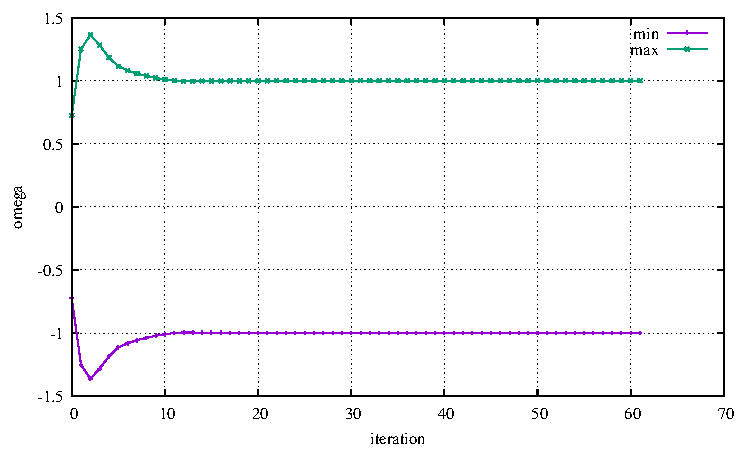
\includegraphics[width=5.7cm]{python_codes/fieldstone_155/stats_omega}\\
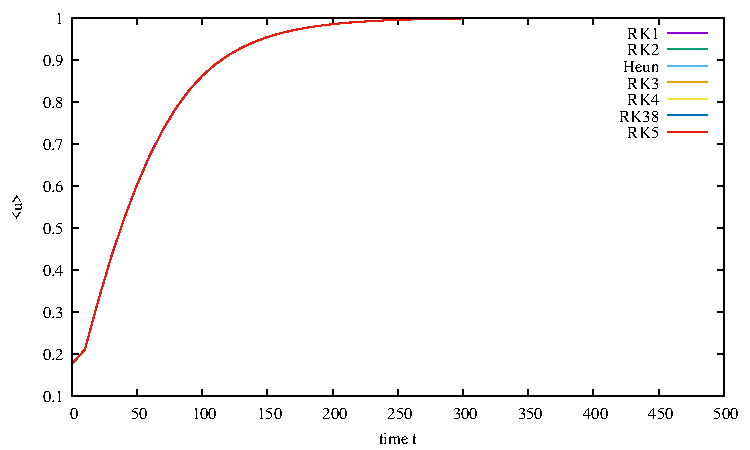
\includegraphics[width=5.7cm]{python_codes/fieldstone_155/avrg_u}
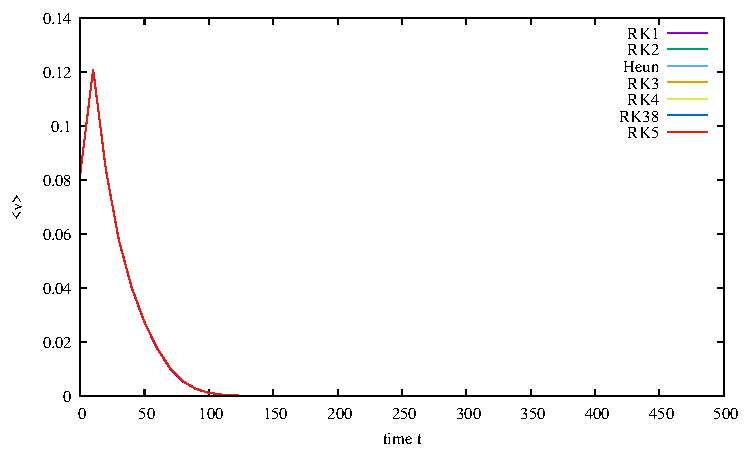
\includegraphics[width=5.7cm]{python_codes/fieldstone_155/avrg_v}
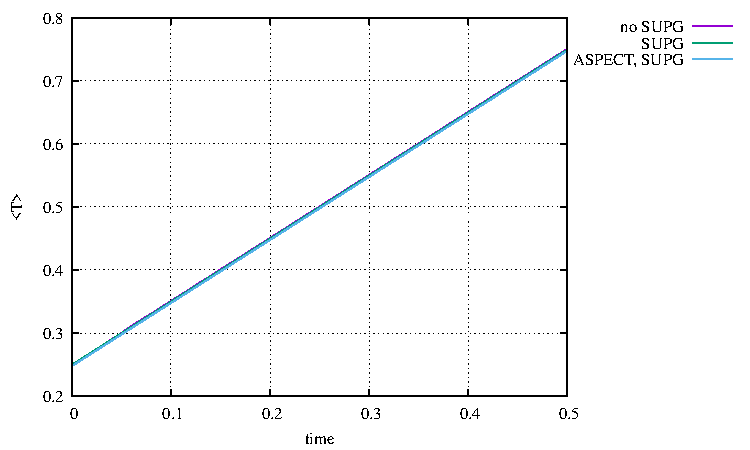
\includegraphics[width=5.7cm]{python_codes/fieldstone_155/avrg_T}\\
\includegraphics[width=5.7cm]{python_codes/fieldstone_155/avrg_psi}
\includegraphics[width=5.7cm]{python_codes/fieldstone_155/avrg_omega}
\end{center}


%%%%%%%%%%%%%%%%%%%%%%%%%%%%%%%%%%%%%%%%%%%%%%%%%%%%%%%%%%%%%%%%%%%%%%%%%%%%%%%%%%%%%%%%%%%%%%%%%%%
\par\noindent\rule{\textwidth}{0.4pt}

\vspace{.5cm}

\begin{center}
\fbox{\begin{minipage}{0.9\textwidth}
{\color{teal}To Do, open questions, future work?}
\begin{itemize}
\item do smthg
\end{itemize}
\end{minipage}}
\end{center}

%%%%%%%%%%%%%%%%%%%%%%%%%%%%%%%%%%%%%%%%%%%%%%%%%%%%%%%%%%%%%%%%%%%%%%%%%%%%%%%%%%%%%%%%%%%%%%%%%%%
\vspace{.5cm}

\Literature:\\
\fullcite{xxxxYY}


